
\section{Additional analysis of calibration convergence}

In the main analysis, each of the 7 chains of the adaptive Metropolis algorithm was initialised by adding random noise around parameter values obtained from a previous calibration. This approach was used to help the algorithm reach the parameter space's areas of high likelihood in a reasonable number of iterations. Indeed, the high number of dimensions ($N=18$) made other approaches such as Latin-Hypercube-based initialisation impractical, as some chains may take millions of iterations before sampling plausible parameter sets.

In a separate experiment, we ran another adaptive Metropolis algorithm where only 10 parameters were varied, but this time initialisation was performed with Latin Hypercube Sampling (LHS) across 10 independent chains. The 10 parameters were selected based on their expected influence on the main findings and whether they were among the primary estimands reported in the manuscript (e.g. face coverings parameter). The remaining 8 parameters were fixed to the maximum a-posteriori value obtained in the main analysis. The aim of this analysis was to verify that the calibration algorithm would recover similar convergence to that obtained in the main analysis despite starting from highly diverse initial points.

Figures \ref{fig:lhs_experiments_likelihood} and \ref{fig:lhs_experiments_traces} illustrate the progression of the parameters during this experiment. The parameter traces were compared against the posterior distributions obtained from the main analysis (Figure \ref{fig:lhs_experiments_traces}). We found that the chains converged to similar values when considering the LHS-based calibration compared to the original analysis. The posterior ranges obtained with the LHS-based analysis were sometimes narrower compared to the original calibration. This can be explained by the fact that more parameters were fixed in the LHS-based calibration than in the original calibration. Consequently, more constraints are imposed on the varied parameters that were previously found to be correlated with parameters that have been fixed in the LHS-based analysis.


\begin{figure}[ht]
    \resizebox{1\textwidth}{!}{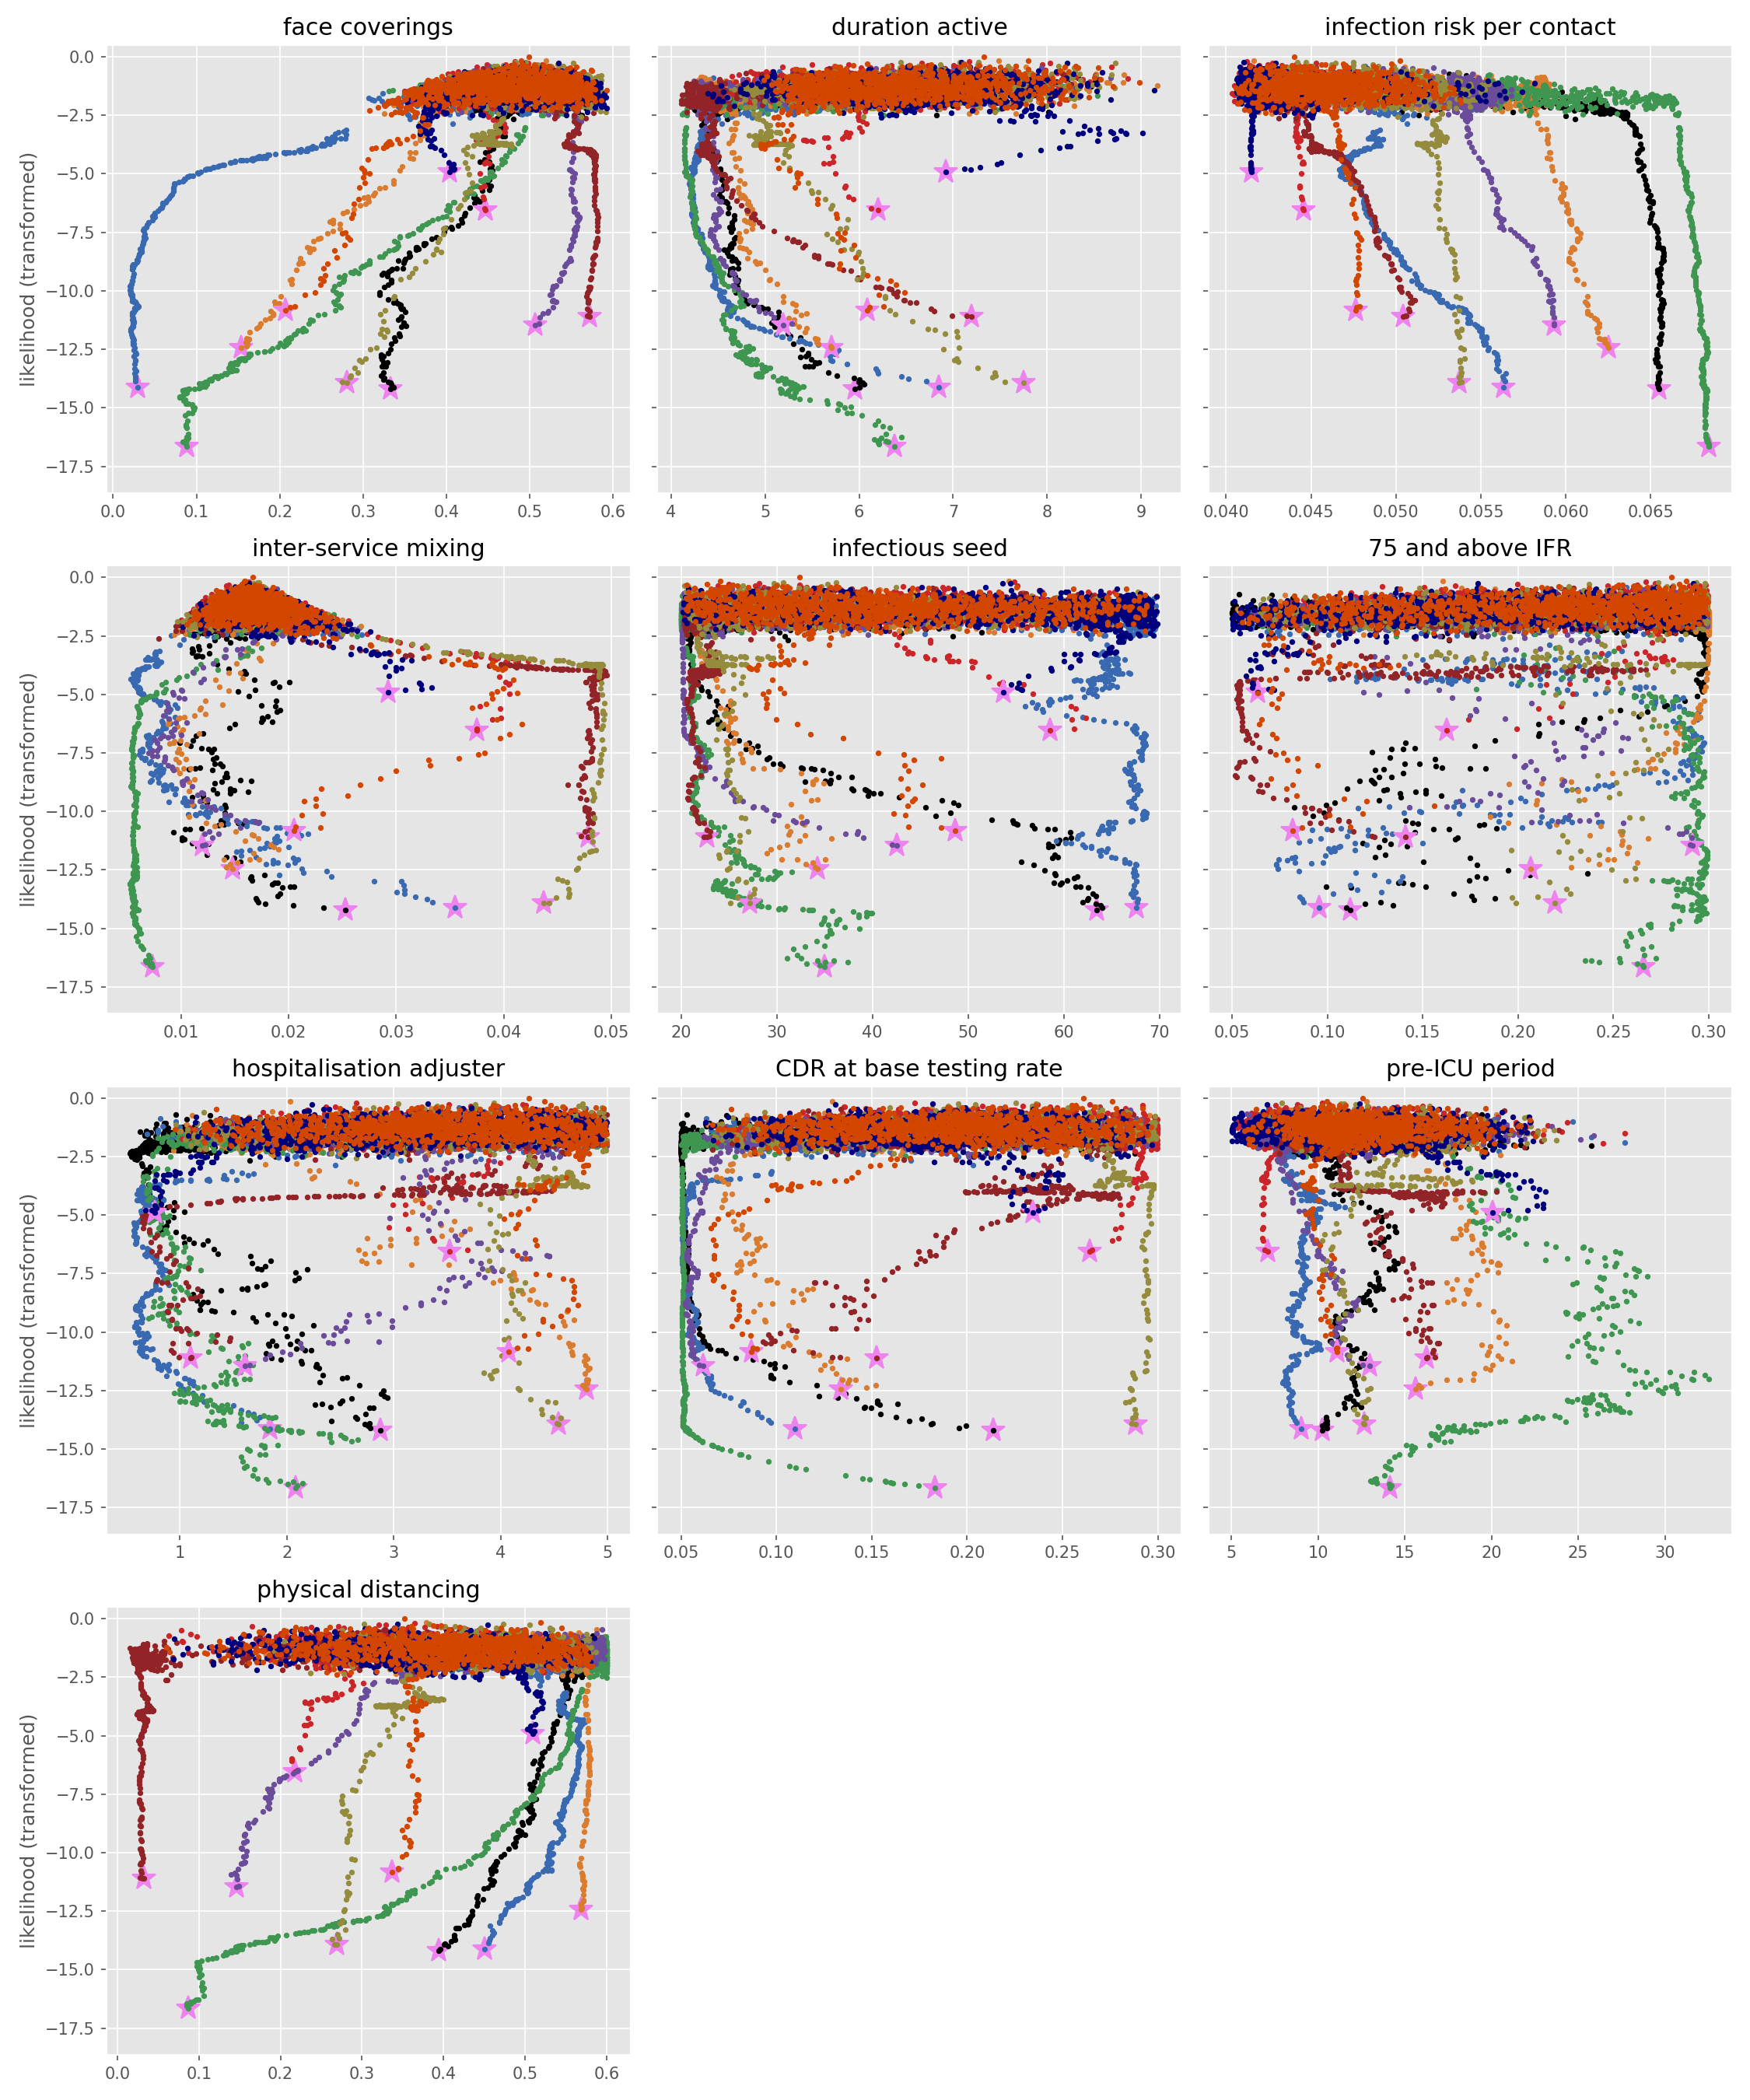
\includegraphics[scale=1]{../covid_19/projects/victoria/lhs_experiments/likelihood_against_params.png}}
    \caption{\textbf{  
	Likelihood against 10 key parameters during calibration initialised with Latin Hypercube Sampling.    
    } 
The different colors represent 10 independent adaptive Metropolis chains initialised with Latin Hypercube Sampling. The likelihood values were transformed to increase clarity using $x \rightarrow -log(-log(x) + m + 1)$, where $m$ is the maximum log-likelihood value. The pink stars highlight the starting points.     
    }
    \label{fig:lhs_experiments_likelihood}
\end{figure}


\begin{figure}[ht]
    \resizebox{1\textwidth}{!}{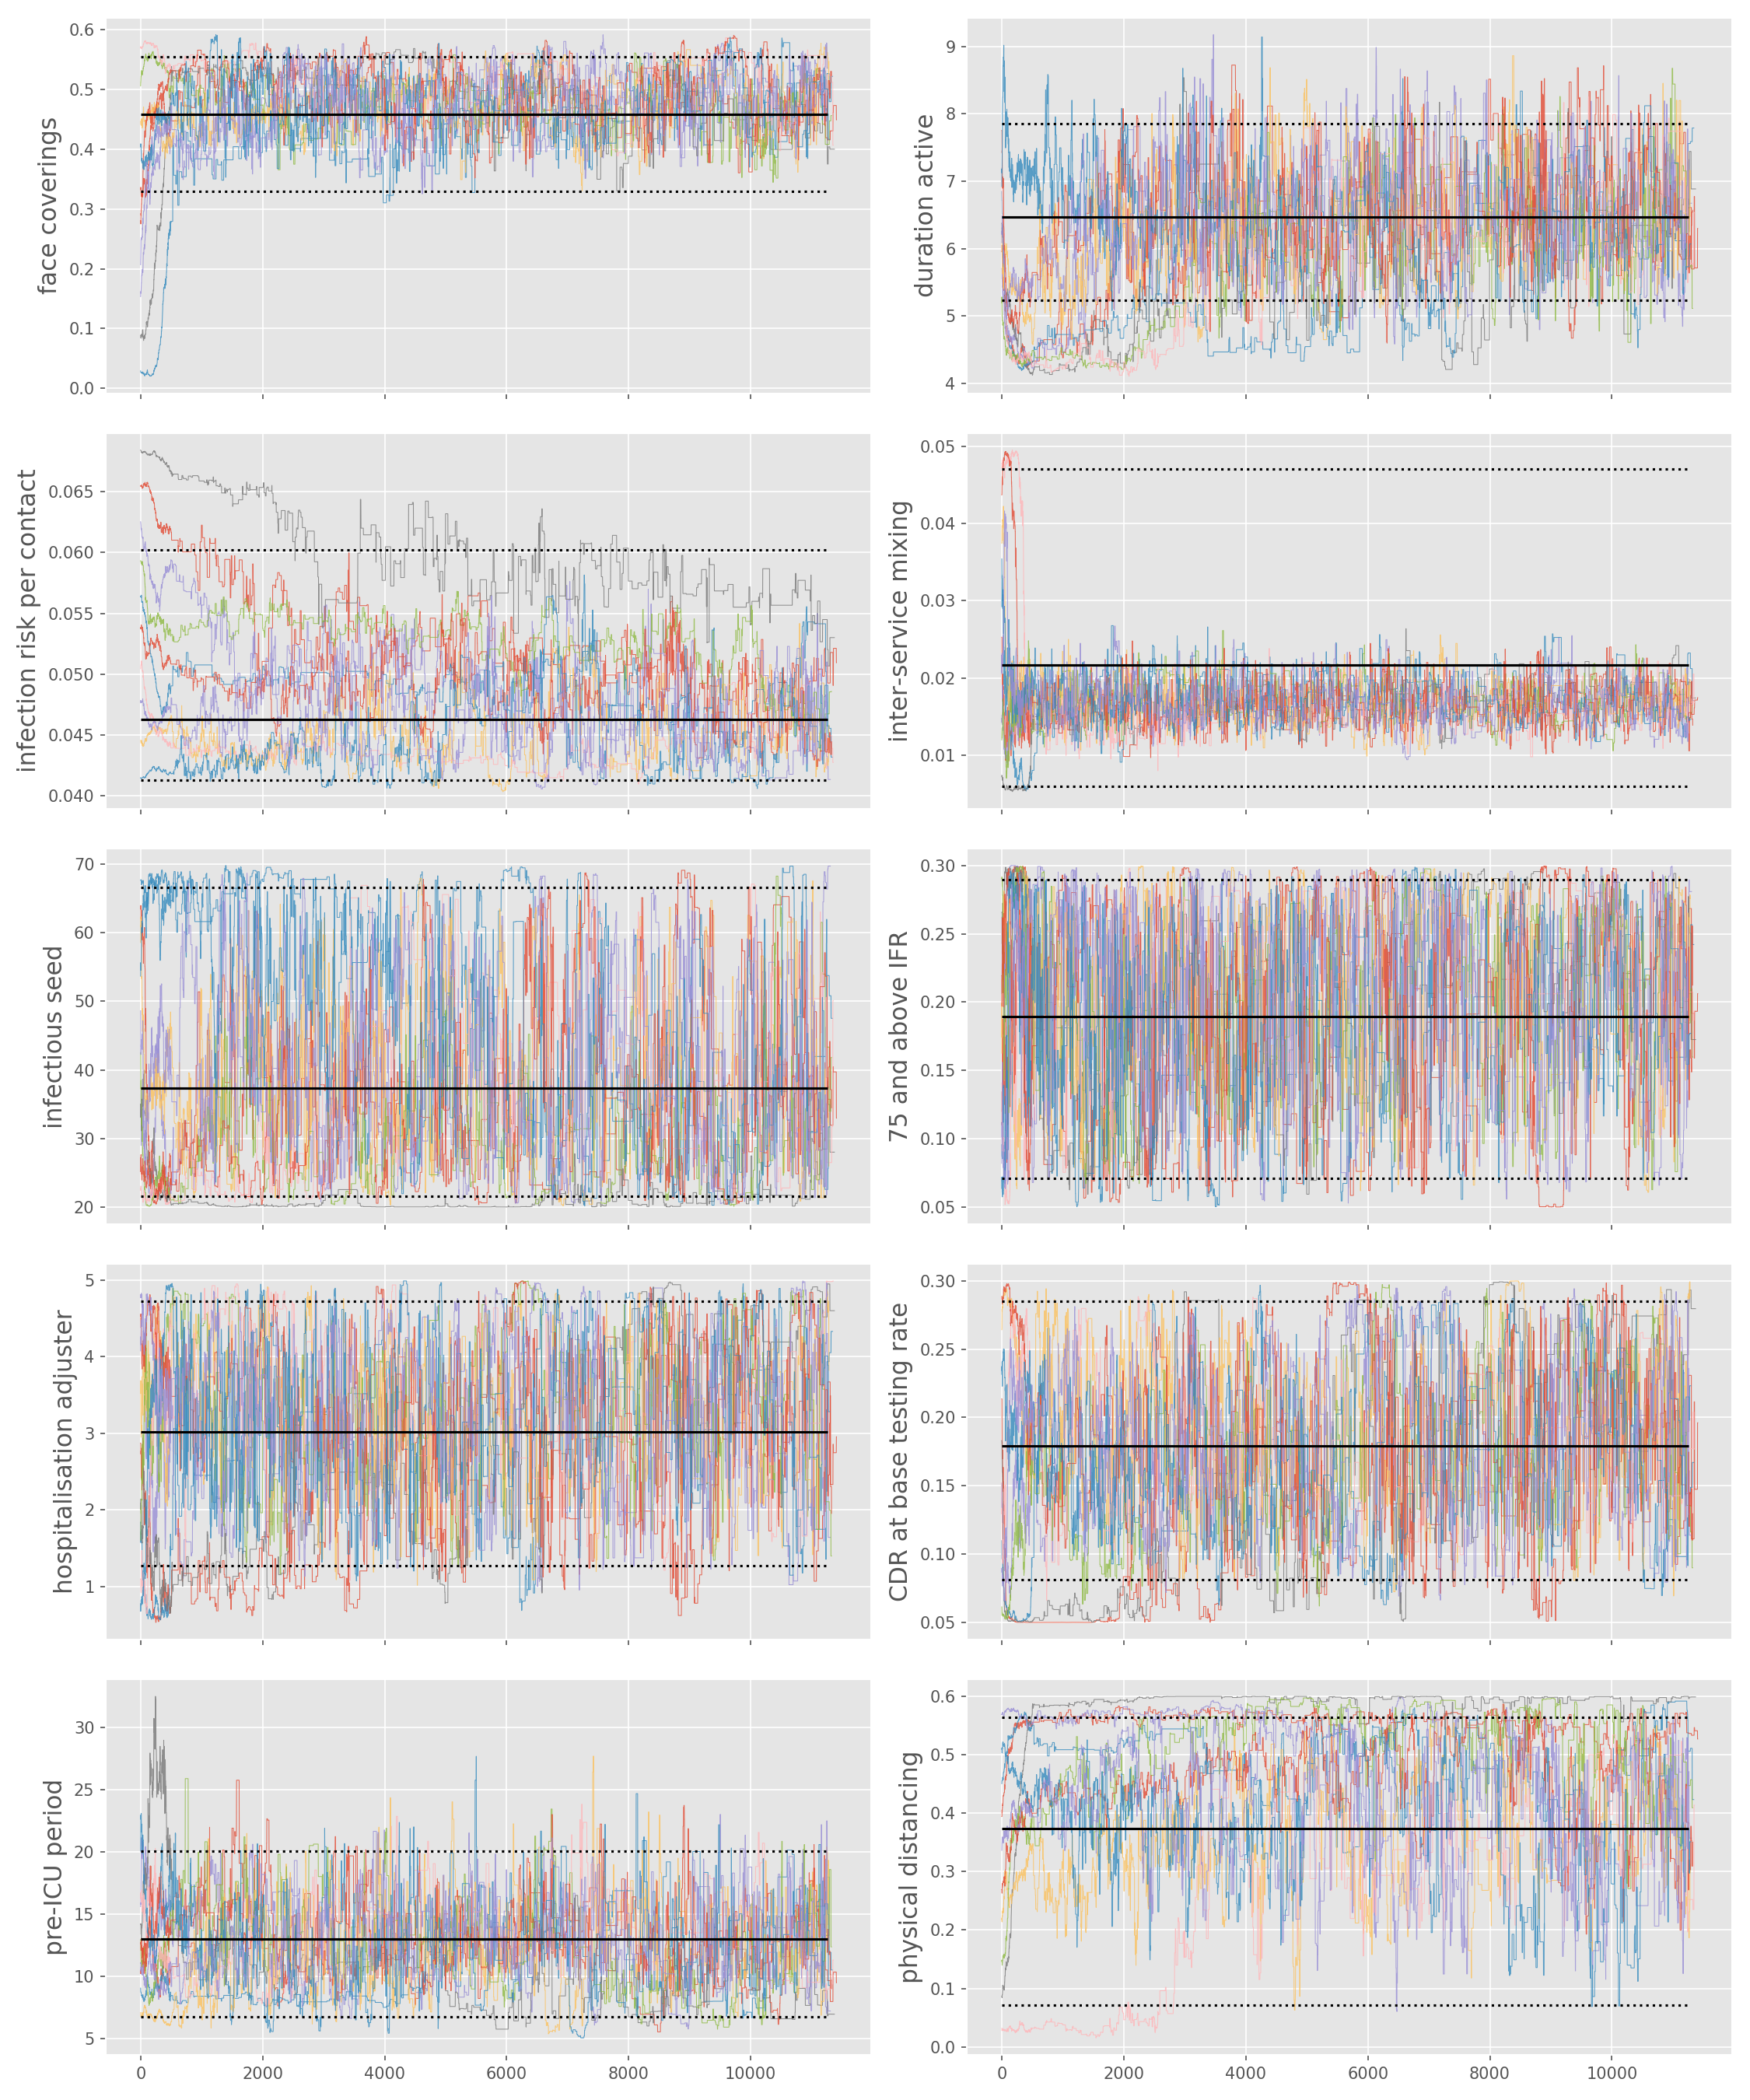
\includegraphics[scale=1]{../covid_19/projects/victoria/lhs_experiments/lhs_start_traces_median.png}}
    \caption{\textbf{Parameter progression traces during calibration initialised with Latin Hypercube Sampling.} The horizontal lines represent the median (solid line) and 95\% credible interval (dotted lines) of the posterior estimates obtained in the main analysis.}
    \label{fig:lhs_experiments_traces}
\end{figure}